\documentclass{article}\usepackage[]{graphicx}\usepackage[]{color}
%% maxwidth is the original width if it is less than linewidth
%% otherwise use linewidth (to make sure the graphics do not exceed the margin)
\makeatletter
\def\maxwidth{ %
  \ifdim\Gin@nat@width>\linewidth
    \linewidth
  \else
    \Gin@nat@width
  \fi
}
\makeatother

\definecolor{fgcolor}{rgb}{0.345, 0.345, 0.345}
\newcommand{\hlnum}[1]{\textcolor[rgb]{0.686,0.059,0.569}{#1}}%
\newcommand{\hlstr}[1]{\textcolor[rgb]{0.192,0.494,0.8}{#1}}%
\newcommand{\hlcom}[1]{\textcolor[rgb]{0.678,0.584,0.686}{\textit{#1}}}%
\newcommand{\hlopt}[1]{\textcolor[rgb]{0,0,0}{#1}}%
\newcommand{\hlstd}[1]{\textcolor[rgb]{0.345,0.345,0.345}{#1}}%
\newcommand{\hlkwa}[1]{\textcolor[rgb]{0.161,0.373,0.58}{\textbf{#1}}}%
\newcommand{\hlkwb}[1]{\textcolor[rgb]{0.69,0.353,0.396}{#1}}%
\newcommand{\hlkwc}[1]{\textcolor[rgb]{0.333,0.667,0.333}{#1}}%
\newcommand{\hlkwd}[1]{\textcolor[rgb]{0.737,0.353,0.396}{\textbf{#1}}}%

\usepackage{framed}
\makeatletter
\newenvironment{kframe}{%
 \def\at@end@of@kframe{}%
 \ifinner\ifhmode%
  \def\at@end@of@kframe{\end{minipage}}%
  \begin{minipage}{\columnwidth}%
 \fi\fi%
 \def\FrameCommand##1{\hskip\@totalleftmargin \hskip-\fboxsep
 \colorbox{shadecolor}{##1}\hskip-\fboxsep
     % There is no \\@totalrightmargin, so:
     \hskip-\linewidth \hskip-\@totalleftmargin \hskip\columnwidth}%
 \MakeFramed {\advance\hsize-\width
   \@totalleftmargin\z@ \linewidth\hsize
   \@setminipage}}%
 {\par\unskip\endMakeFramed%
 \at@end@of@kframe}
\makeatother

\definecolor{shadecolor}{rgb}{.97, .97, .97}
\definecolor{messagecolor}{rgb}{0, 0, 0}
\definecolor{warningcolor}{rgb}{1, 0, 1}
\definecolor{errorcolor}{rgb}{1, 0, 0}
\newenvironment{knitrout}{}{} % an empty environment to be redefined in TeX

\usepackage{alltt}
\usepackage[sc]{mathpazo}
\renewcommand{\sfdefault}{lmss}
\renewcommand{\ttdefault}{lmtt}
\usepackage[T1]{fontenc}
\usepackage{geometry}
\geometry{verbose,tmargin=2.5cm,bmargin=2.5cm,lmargin=2.5cm,rmargin=2.5cm}
\setcounter{secnumdepth}{2}
\setcounter{tocdepth}{2}
\usepackage[unicode=true,pdfusetitle,
 bookmarks=true,bookmarksnumbered=true,bookmarksopen=true,bookmarksopenlevel=2,
 breaklinks=false,pdfborder={0 0 1},backref=false,colorlinks=false]
 {hyperref}
\hypersetup{
 pdfstartview={XYZ null null 1}}

\makeatletter
%%%%%%%%%%%%%%%%%%%%%%%%%%%%%% User specified LaTeX commands.
\renewcommand{\textfraction}{0.05}
\renewcommand{\topfraction}{0.8}
\renewcommand{\bottomfraction}{0.8}
\renewcommand{\floatpagefraction}{0.75}

\makeatother
\IfFileExists{upquote.sty}{\usepackage{upquote}}{}
\begin{document}








The results below are generated from an R script.

\begin{knitrout}
\definecolor{shadecolor}{rgb}{0.969, 0.969, 0.969}\color{fgcolor}\begin{kframe}
\begin{alltt}
\hlcom{#NDVI percent N plots and non-linear curve fits}

\hlcom{#reading in the data}
\hlkwd{setwd}\hlstd{(}\hlstr{'~/Data/'}\hlstd{)}
\hlkwd{dir}\hlstd{()}
\end{alltt}
\begin{verbatim}
## [1] "Lonely_2012and2013_spec_biomass_NDVI_Base.xlsx"     
## [2] "lonely_cn.csv"                                      
## [3] "Lonely_N_and_C_data_for_spec_analysis_12_21_15.xlsx"
## [4] "Lonelybiomassndvi.csv"                              
## [5] "VegPlots_for R.csv"                                 
## [6] "VegPlots_for R.xlsx"                                
## [7] "VegPlotSum_11_12_13_14_15_MeansCombo_eMODIS.xlsx"
\end{verbatim}
\begin{alltt}
\hlcom{#csv file cleaned up by Dan.}
\hlcom{#need to compare to original data file- confirm that removing na's in kyle's analysis resulted in consistent dataset being used for all models compared w/ AIC.}
\hlstd{vegplots}\hlkwb{<-}\hlkwd{read.csv}\hlstd{(}\hlstr{'VegPlots_for R.csv'}\hlstd{)}

\hlcom{#load phenology curve functions}
\hlkwd{source}\hlstd{(}\hlstr{'../code/phenolcurve.r'}\hlstd{)}
\hlkwd{source}\hlstd{(}\hlstr{'../code/aic_code.r'}\hlstd{)}
\hlkwd{library}\hlstd{(AICcmodavg)}
\hlkwd{library}\hlstd{(MASS)} \hlcom{#fitdistr function in MASS allows one to fit good parameters.}
\hlkwd{library}\hlstd{(minpack.lm)}
\hlkwd{library}\hlstd{(ggplot2)}

\hlcom{####################################################################}
\hlcom{#ggplot scatter plots to look at variation in %N and ndvi over season and by year.}
\hlcom{#install ggplot2 if necessary}
\hlstd{vegplots}\hlopt{$}\hlstd{Yr.fac}\hlkwb{<-}\hlkwd{as.factor}\hlstd{(vegplots}\hlopt{$}\hlstd{Yr)} \hlcom{#making year a grouping factor.}

\hlcom{#ndvi over season, by year}
\hlcom{#- using worldview2 ndvi from specrad readings.}
\hlcom{#bmp('../output_plots/emo_ndvi_season_year.bmp',height=480,width=640)}
\hlstd{eMO.ndvi.plot}\hlkwb{<-}\hlkwd{ggplot}\hlstd{(}\hlkwc{dat}\hlstd{=vegplots,} \hlkwd{aes}\hlstd{(}\hlkwc{x}\hlstd{=DOY,}\hlkwc{y}\hlstd{=eMO_NDVI,}\hlkwc{color}\hlstd{=Yr.fac))}\hlopt{+}\hlkwd{geom_point}\hlstd{()}\hlopt{+}\hlkwd{geom_smooth}\hlstd{()}
\hlstd{eMO.ndvi.plot}
\end{alltt}
\end{kframe}

{\centering 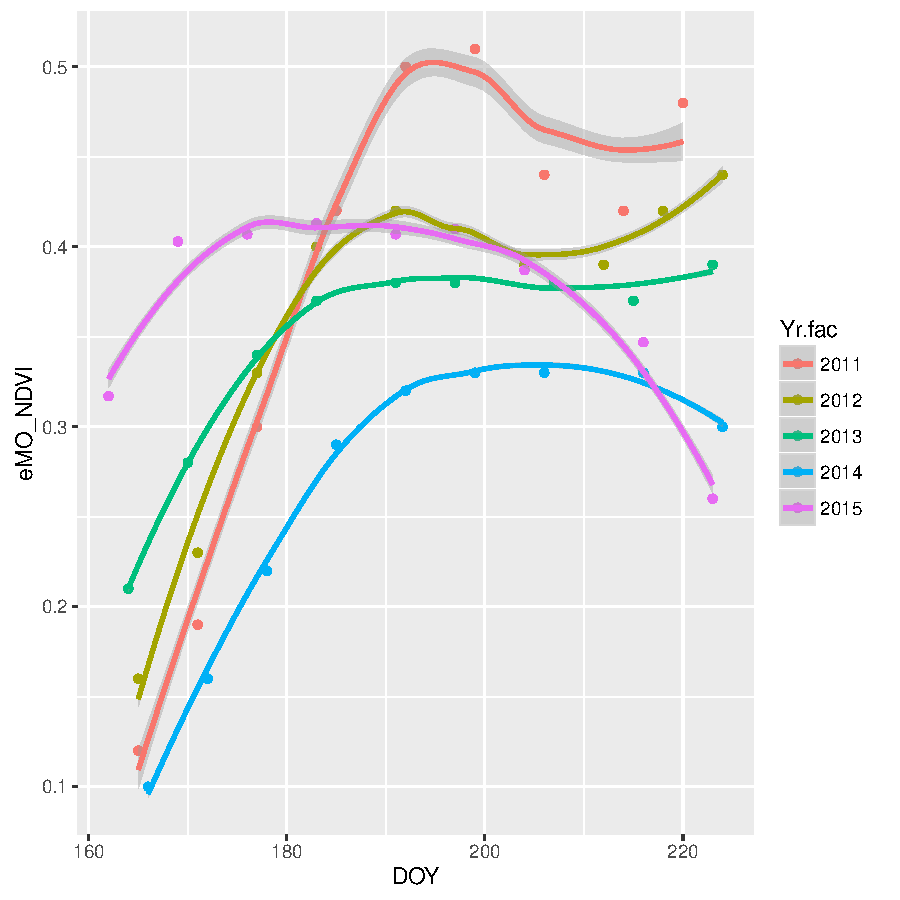
\includegraphics[width=.6\linewidth]{figure/ndvi-pn-phenol-stitchtest-Rnwauto-report-1} 

}


\begin{kframe}\begin{alltt}
\hlcom{#dev.off()}
\hlcom{#asymptote with gradual decline on the right side.}

\hlcom{#% N over season, by Year}
\hlcom{#bmp('../output_plots/pctN_season_year.bmp',height=480,width=640)}
\hlstd{pN.plot}\hlkwb{<-}\hlkwd{ggplot}\hlstd{(}\hlkwc{dat}\hlstd{=vegplots,} \hlkwd{aes}\hlstd{(}\hlkwc{x}\hlstd{=DOY,}\hlkwc{y}\hlstd{=PrcntN,}\hlkwc{color}\hlstd{=Yr.fac))}\hlopt{+}\hlkwd{geom_point}\hlstd{()}\hlopt{+}\hlkwd{geom_smooth}\hlstd{()}
\hlstd{pN.plot}
\end{alltt}


{\ttfamily\noindent\color{warningcolor}{\#\# Warning: Removed 154 rows containing non-finite values (stat\_smooth).}}

{\ttfamily\noindent\color{warningcolor}{\#\# Warning: Removed 154 rows containing missing values (geom\_point).}}\end{kframe}

{\centering 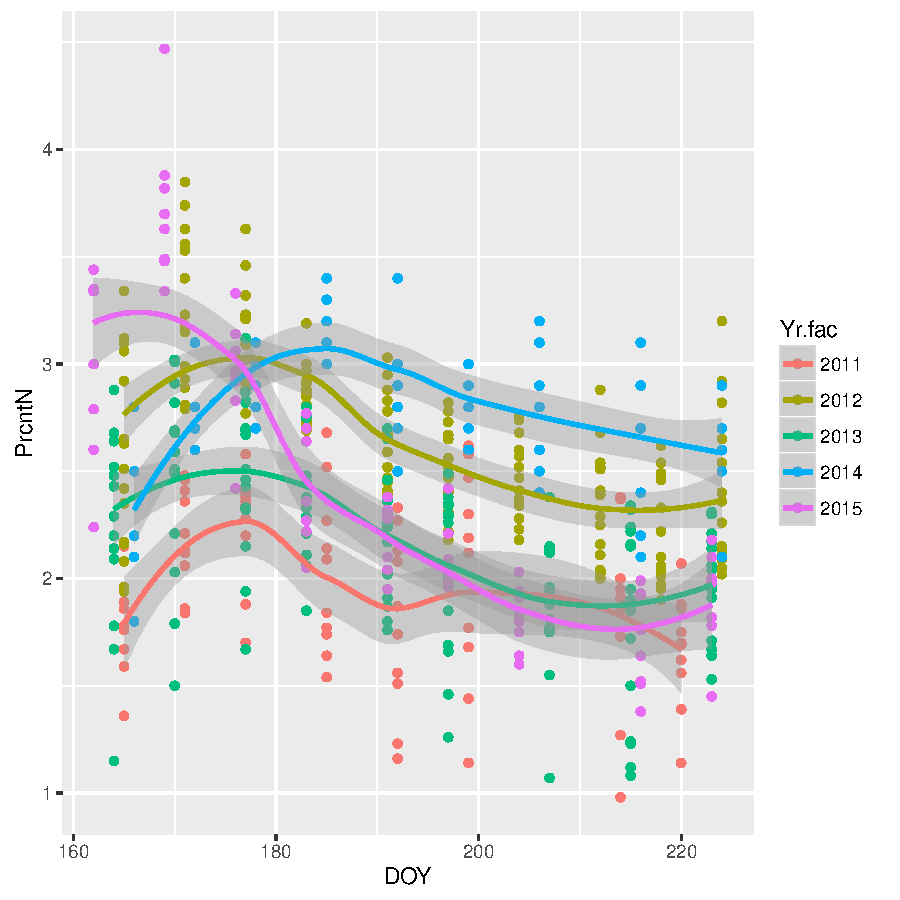
\includegraphics[width=.6\linewidth]{figure/ndvi-pn-phenol-stitchtest-Rnwauto-report-2} 

}


\begin{kframe}\begin{alltt}
\hlcom{#dev.off()}
\hlcom{#looks like a right-tailed curve.}
\end{alltt}
\end{kframe}
\end{knitrout}

The R session information (including the OS info, R version and all
packages used):

\begin{knitrout}
\definecolor{shadecolor}{rgb}{0.969, 0.969, 0.969}\color{fgcolor}\begin{kframe}
\begin{alltt}
\hlkwd{sessionInfo}\hlstd{()}
\end{alltt}
\begin{verbatim}
## R version 3.2.0 (2015-04-16)
## Platform: x86_64-w64-mingw32/x64 (64-bit)
## Running under: Windows 7 x64 (build 7601) Service Pack 1
## 
## locale:
## [1] LC_COLLATE=English_United States.1252  LC_CTYPE=English_United States.1252   
## [3] LC_MONETARY=English_United States.1252 LC_NUMERIC=C                          
## [5] LC_TIME=English_United States.1252    
## 
## attached base packages:
## [1] stats     graphics  grDevices utils     datasets  methods   base     
## 
## other attached packages:
## [1] knitr_1.11       ggplot2_2.0.0    minpack.lm_1.2-0 MASS_7.3-45      AICcmodavg_2.0-3
## 
## loaded via a namespace (and not attached):
##  [1] Rcpp_0.12.2      raster_2.5-2     magrittr_1.5     splines_3.2.0    munsell_0.4.2   
##  [6] colorspace_1.2-6 xtable_1.8-0     lattice_0.20-31  highr_0.5.1      stringr_1.0.0   
## [11] plyr_1.8.3       tools_3.2.0      grid_3.2.0       unmarked_0.11-0  nlme_3.1-120    
## [16] gtable_0.1.2     digest_0.6.8     Matrix_1.2-0     formatR_1.2.1    evaluate_0.8    
## [21] VGAM_1.0-0       labeling_0.3     sp_1.2-1         stringi_1.0-1    scales_0.3.0    
## [26] stats4_3.2.0     reshape_0.8.5
\end{verbatim}
\begin{alltt}
\hlkwd{Sys.time}\hlstd{()}
\end{alltt}
\begin{verbatim}
## [1] "2015-12-28 11:49:46 AKST"
\end{verbatim}
\end{kframe}
\end{knitrout}


\end{document}
